\section{Stato dell'Arte}

\subsection{Epidemiologia}
L'epidemiologia è la disciplina biomedica che studia la 
distribuzione e la frequenza delle malattie ed eventi di 
rilevanza sanitaria nella popolazione.
Si occupa di analizzare le cause, il decorso e le 
conseguenze delle malattie.\cite{Galea2009-lj} \cite{Parascandola2001-kw}

L'epidemiologia è una disciplina molto pratica, che visto 
l'obiettivo che si pone, ovvero quello di trovare le cause
relative ad un dato effetto, non può esentarsi dagli 
svariati problemi che gravitano e definiscono questo 
nobile obiettivo, primo tra tutti: cosa vuol dire che un
evento è causa di un altro e come definisco questo 
tipo di rapporto in maniera inequivocabile?

Questi interrogativi possono sembrare banali in quanto 
come specie ci siamo evoluti per trovare una correlazione
di causalità tra eventi anche quando questi non ne hanno.
Ad esempio se fossimo in un bosco, al buio e soli con
l'unico rumore ad accompagnarci che è quello di una 
piacevole brezza estiva, se percepissimo un rumore tra 
i cespugli, molto probabilmente penseremmo che c'è 
qualcosa che non va, che ci sia un pericolo in agguato,
un predatore, anche se magari la motivazione è 
la suddetta brezza. 

Questo adattamento evolutivo ci ha permeso di sopravvivere
in situazioni di pericolo, ma sfortunatamente quando 
si parla di scienza e di dati, non sempre l'istinto è 
qualcosa a cui affidarsi, in quanto i dati di
per loro non dicono assolutamente nulla, siamo noi 
in quanto individui dotati di intelletto, tecniche e metodi a dover
estrapolare dei significati che verifichiamo essere corretti e inequivocabili.

Se ci soffermiamo su questa ultima affermazione, possiamo
essere facilmente tratti in inganno. Prendiamo per esempio 
il seguente grafico che mostra in maniera \emph{inequivocabile} 
come la spesa da parte degli USA sulla ricerca aerospaziale sia 
direttamente collegata al numero di suicidi per strangolamento. 

\begin{figure}[h]
    \begin{center}
        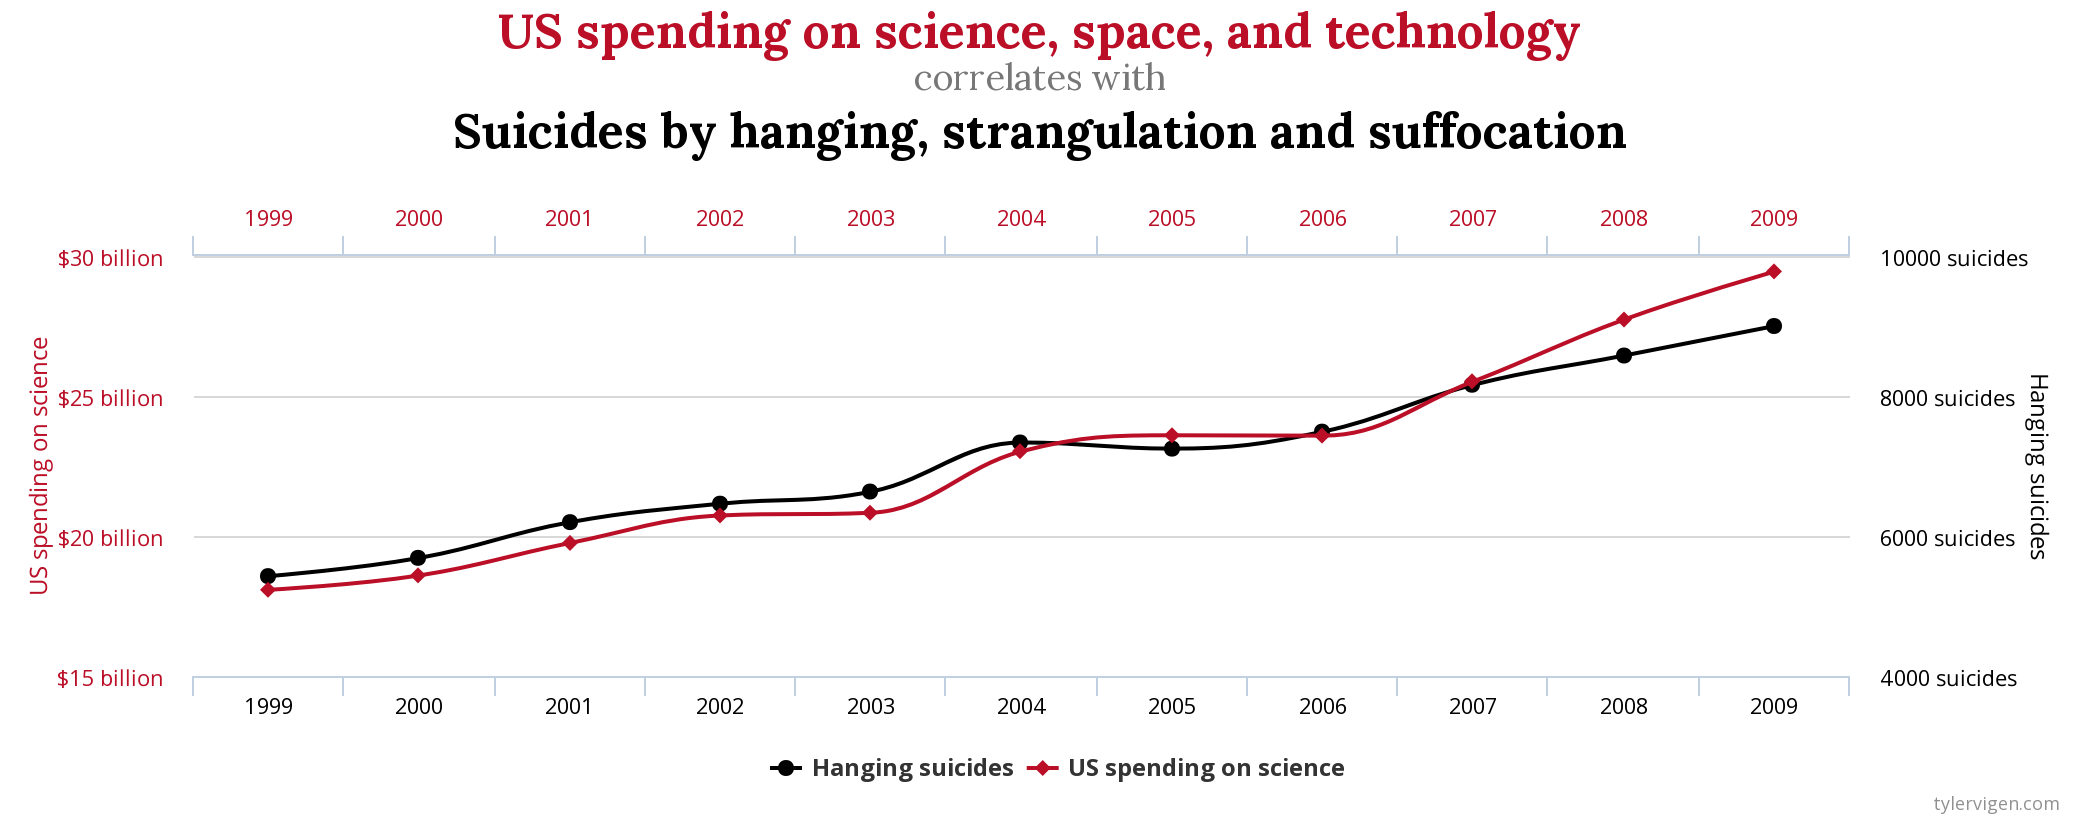
\includegraphics[width=\linewidth]{img/chart.png}
        \caption{Esempio di correlazione spuria}
        \url{https://www.tylervigen.com/spurious-correlations}
        \label{fig:spurious_relations}
    \end{center}
\end{figure}

Affidandoci solamente al grafico e ai dati riportati in 
figura, ci verrebbbe da pensare che le due categorie 
siano in qualche modo correlate, e che il governo 
americano debba essere fermato, in quanto respondabile di 
incitamento al suicidio.
Ebbene non è così, questo è un caso di \textbf{relazione 
spuria}, ovvero che due o 
più variabili sono associate ma non causalmente correlate.

Associatività e causalità infatti non sono la stessa cosa,
ed è bene quando si studia l'una, non confondersi con l'altra.
In statistica, una correlazione tra dati è una qualsiasi 
relazione che vi è tra due o più variabili, sia essa di 
tipo causale oppure non. 
Nell'esempio di prima la correlazione
tra le due variabili potrebbe essere banalmente il tempo, 
infatti con il passare del tempo la spesa media per la 
ricerca aerospaziale è continuata a salire per via 
del sempre più alto interesse e investimento nel settore
e sfortunatamente con il passare degli anni si è registrato
un aumento costante del numero di suicidi. 

Il \textbf{bias} che abbiamo verso la ricerca di un intreccio
tra gli eventi, in maniera che questi siano sempre contigui
l'uno con l'altro, in maniera che si possa tracciare una 
chiara e distinta linea dal primo all'ultimo ci trae in 
inganno quando questi sembrano esserlo ma in realtà non lo sono.
Molto spesso la risposta più semplice è anche quella meno 
interessante, benchè corretta, ovvero che due eventi 
completamente slegati tra loro possono avere andamenti simili, 
così come differenti addendi possono portare lo stesso risultato; 

\begin{figure}[h]
    \begin{center}
        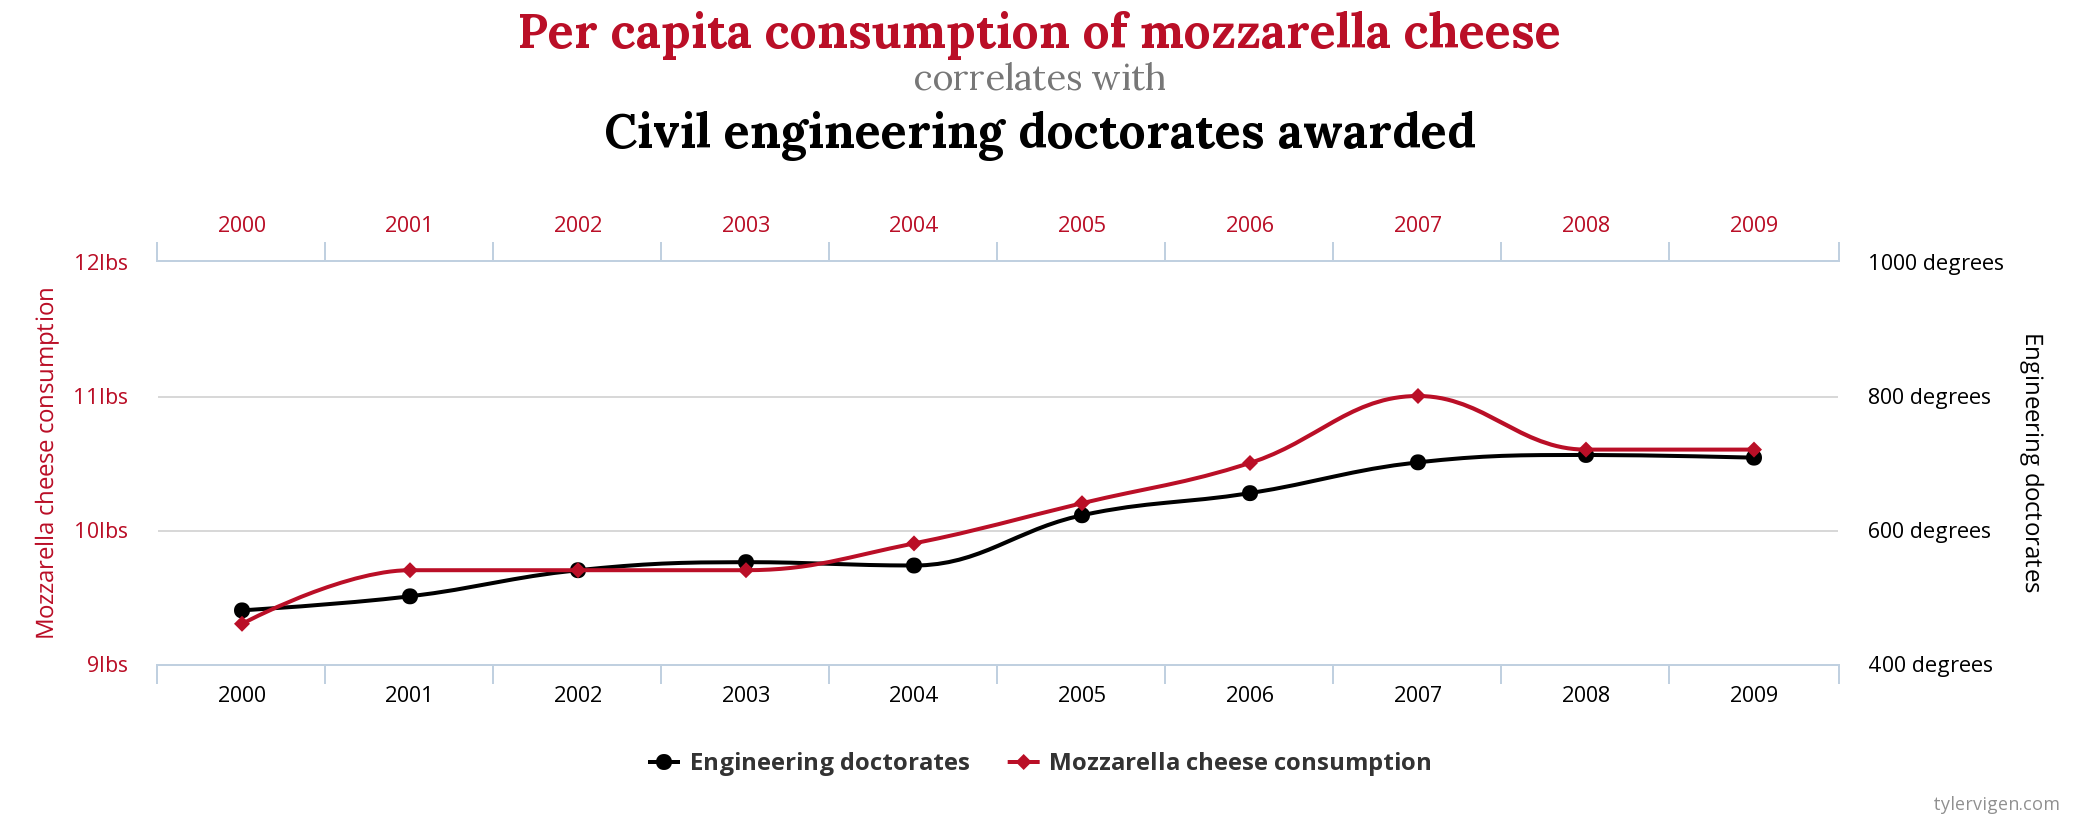
\includegraphics[width=\linewidth]{img/chart1.png}
        \caption{Un altro esempio di correlazione spuria}
        \url{https://www.tylervigen.com/spurious-correlations}
        \label{fig:another_spurious_relations}
    \end{center}
\end{figure}

\newpage

Il problema della causalità non è da prendere sotto gamba
ed è uno dei problemi cardine quando si vogliono determinare e 
applicare degli intervanti all'interno di una popolazione per
cercare di mitigare ad esempio la diffusione di un agente 
patogeno \cite{Parascandola2001-kw}. 

Come è stato già introdotto precedentemente, i dati di per loro
non dicono nulla, siamo noi che dobbiamo imparare a 
capire il significato di ciò che esprimono. Un esempio 
estremamente calzante di come pur avendo bene in mente il
problema sopra citato delle correlazioni \emph{spurie}, si
possa comunque essere ingannati dai dati, è il seguente:

Poniamo di essere un medico e di dover decidere se 
prescrivere o meno ad un paziente un determinato medicinale.
Per aiutarci nella decisione abbiamo la storia clinica
del paziente e i risultati di uno studio su una nuova 
medicina che attesta di curare il malessere del paziente.
Questa nuova medicina è stata testata su un gruppo di 
settecento persone divise in due pari sottogruppi in cui 
350 pazienti decidevano autonomamente se prendere o meno 
la medicina e 350 decidevano autonomamente il contrario.
I risultati sono i seguenti:

\begin{tabular}{ |p{2,2cm}||p{1,6cm}|p{1,6cm}|p{1,6cm}||p{1,6cm}|p{1,6cm}|p{1,6cm}|  }
	\hline
	\multicolumn{7}{|c|}{Simpson's paradox} \\
	\hline
	Category & Patients & Recovered & \% Recovered & Patients & Recovered & \% Recovered\\
	\hline
	Men & 87 & 81 & 93\% & 270 & 234 & 87\% \\
	Women & 263 & 192 & 73\% & 80 & 55 & 69\% \\
    Combined data & 350 & 273 & 78\% & 350 & 289 & 83\% \\
	\hline
\end{tabular}

Questi risultati sembrano suggerire come la prescrizione 
di questa nuova medicina non aiuti i pazienti a stare meglio.
Tuttavia questo risultato cade nel così detto \emph{paradosso di Simpson}
per cui i dati aggregati relativi 
ad uno specifico trattamento sembrano descrivere una sua 
perdita di efficacia relativamente ai singoli dati delle 
singole categorie in esame, portando un lettore non attento 
a cadere nell'inganno di pensare che ci sia una perdita di 
efficacia. Questo esempio pone l'accento sul fatto che non sempre
estrapolare informazioni da dei dati aggregati può risultare
efficace, e anzi, alle volte questi possono ingannare.
In questi casi bisogna estrapolare le informazioni di 
causalità dai dati singoli.

è chiaro che non sia così semplice comprendere le cause 
di un determinato effetto, o insieme di effetti. Conoscere
l'agente patogeno, o quanto meno la sua natura può aiutare,
ma non sempre è sufficiente. L'utilizzo di modelli di 
Machine Learning per l'estrapolazione di dati, di correlazioni
e successivamente per la definizione di policy di intervento
può risultare in un rischio non indifferente ma al contempo 
descrive un potente alleato per la definizione di policy di 
intervento all'interno di settori estremamente delicati come 
quelli sanitari \cite{doi:10.1098/rsos.220638}.